\documentclass{standalone}
\usepackage{tikz}
\usetikzlibrary{arrows.meta}
\tikzset{label/.style = {inner sep=1pt, fill=white}}
%\tikzset{nd/.style={circle, inner sep=0pt}}
\tikzset{nd/.style={inner sep=1pt}}
\tikzset{>=Latex}
\tikzset{arc/.style = {->, semithick, >=Latex}}
\begin{document}
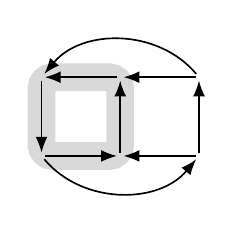
\begin{tikzpicture}

    \node[nd] (1) at (0,0) {};
    \node[nd] (2) at (0,1) {};
    \node[nd] (3) at (1,0) {};
    \node[nd] (4) at (1,1) {};
    \node[nd] (5) at (2,0) {};
    \node[nd] (6) at (2,1) {};

    \draw [rounded corners, color = gray!30, line width = 10pt] (0,0) to (0,1) to (1,1) to (1,0) to cycle;
    
    \draw[arc] (1) to (3);
    \draw[arc] (1) to[out = -50, in = -130] (5);
    \draw[arc] (6) to[out = 130, in = 50] (2);
    \draw[arc] (5) to (3);
    \draw[arc] (4) to (2);
    \draw[arc] (6) to (4);
    
    \draw[arc] (5) to (6);
    \draw[arc] (3) to (4);
    \draw[arc] (2) to (1);
 \end{tikzpicture}
\end{document}